% Author : Ali Snedden
% Date   : 9/10/19
% Compile:
%   pdflatex -shell-escape nerd_hour_09_13_2019.tex


\documentclass{beamer}
%\usetheme{Ilmenau}
\usetheme{Copenhagen}
%\usecolortheme{seahorse}
% See http://www.hartwork.org/beamer-theme-matrix/ for more themes and colors

% for themes, etc.
%\mode<presentation>{ \usetheme{boxes} }
%\mode<presentation>{ \usetheme{Warsaw} }
%\renewcommand*{\bibfont}{\scriptsize}

\usepackage{times}  % fonts are up to you
\usepackage{graphics}
\usepackage{amsmath}
\usepackage[makeroom]{cancel}
\usepackage{media9}
\usepackage{hyperref}
\usepackage{movie15}
\usepackage{epstopdf}

\usepackage{tikz}
\usetikzlibrary{fit}

\usepackage[absolute,overlay]{textpos}
\usepackage{psfrag}

%http://tex.stackexchange.com/questions/302584/problems-related-to-beamer-footcite
\makeatletter
\def\@iiiminipage#1#2[#3]#4{%
    \leavevmode
    \@pboxswfalse
    \setlength\@tempdima{#4}%
    \def\@mpargs{{#1}{#2}[#3]{#4}}%
    \setbox\@tempboxa\vbox\bgroup
    \color@begingroup
    \hsize\@tempdima
    \textwidth\hsize \columnwidth\hsize
    \@parboxrestore
    \let\@footnotetext\@mpfootnotetext
    \let\@listdepth\@mplistdepth \@mplistdepth\z@
    \@minipagerestore
    \@setminipage}
\makeatother

%http://tex.stackexchange.com/questions/138744/how-do-i-remove-citation-number-from-footcite
%\newcommand\footcitenonum[1]{%
%  \begingroup
%  \renewcommand\thefootnote{}\footnote{#1}%
%  \addtocounter{footnote}{-1}%
%  \endgroup
%}
%
%\makeatletter
%\renewrobustcmd{\blx@mkbibfootnote}[2]{%
%  \iftoggle{blx@footnote}
%    {\blx@warning{Nested notes}%
%     \addspace\mkbibparens{#2}}
%    {\unspace
%     \ifnum\blx@notetype=\tw@
%       \expandafter\@firstoftwo
%     \else
%       \expandafter\@secondoftwo
%     \fi
%       {\csuse{blx@theendnote#1}{\protecting{\blxmkbibnote{end}{#2}}}}
%       {\csuse{footnotenonum#1}{\protecting{\blxmkbibnote{foot}{#2}}}}}}
%\makeatother

%Bibliography stuff
%\usepackage[style=verbose,autocite=footnote,maxnames=10,babel=hyphen,hyperref=true,abbreviate=false,backend=biber,mcite]{biblatex}

\usepackage[style=authoryear]{biblatex}
%\usepackage[bottom]{footmisc}
%\bibliography{/Users/asnedden/Library/texmf/bibtex/bib/references}
\addbibresource{/Users/asnedden/Library/texmf/bibtex/bib/references.bib}
%\bibliographystyle{apj}
\setbeamertemplate{bibliography item}[text]
%\usepackage[backend=bibtex, style=authoryear]{biblatex}
%\addbibresource{/Users/ali/Library/texmf/bibtex/bib/references.bib}
\newcommand{\customcite}[1]{\citeauthor{#1}, \citeyear{#1}}
\renewcommand*{\bibfont}{\tiny}

\usefonttheme[onlymath]{serif}

\newcommand\smallFont{\fontsize{8}{7.2}\selectfont}   %Change font size.
\newcommand\mCite[1]{[\cite{#1}, \citetitle{#1}]}  %Prints name and title
\newcommand\FrameText[1]{
\begin{textblock*}{\paperwidth}(0pt,\textheight)
    \vspace{1.0cm}
    \raggedleft \smallFont #1
\end{textblock*}}


%Get rid of ugly copenhagen default symbol for enumerate
\setbeamertemplate{enumerate items}[default]   

%Increase default separation size between items in itemize and enumerate 

\tikzset{type1/.style={rectangle, rounded corners, minimum width=3cm, minimum height=0.1cm,text centered, draw=black, fill=blue!10, text width=2cm},
        type2/.style={rectangle, rounded corners, minimum width=3cm, minimum height=0.1cm, text centered, draw=black, fill=blue!10, text width=5cm},
        info/.style = {rectangle, rounded corners, minimum width=2.5cm, minimum height=0.1cm, text centered, draw=black, 
            fill=blue!30, text width=2.5cm},
        org/.style={rectangle, rounded corners, minimum width=2cm, minimum height=0.1cm, text centered, draw=black, 
            fill=blue!30, text width=3cm},
        decision/.style = {square, minimum width=1cm, minimum height=0.1cm, text centered, 
            draw=black, fill=green!30, text width=4cm},
        arrow/.style = {thick,->,>=stealth},
    }
    
    
    
   

%%%%%%%%%%%%%%% BIBLIOGRAPHY COMMANDS %%%%%%%%%%%%%%%
\newcommand{\apj}{ApJ.}
\newcommand{\apjs}{ApJS}
\newcommand{\apjl}{ApJL}
\newcommand{\pasp}{Publications of the Astronomical Society of the Pacific}
\newcommand{\pasj}{Publ. of the Astron. Soc. of Japan}
\newcommand{\prc}{Phys. Rev. C}
\newcommand{\prd}{Phys. Rev. D}
\newcommand{\nat}{Nature}
\newcommand{\mnras}{Mon. Not. R. Astron. Soc.}
\newcommand{\na}{New Astronomy}
\newcommand{\aap}{Astronomy and Astrophysics}
\newcommand{\araa}{Annu. Rev. Astron. Astrophys}
\newcommand{\aj}{Astronomical Journal}
\newcommand{\pasa}{Pub. of the Astron. Soc. of Australia}
\newcommand{\nar}{New Astronomy Reviews}


%%%%%%%%%%%%%%% OTHER COMMANDS %%%%%%%%%%%%%%%%%
\newcommand{\subitem}{\item[$-$]}


% these will be used later in the title page
\title{Ripples in the Universe : Black hole and Neutron Star mergers}
\author{Ali Snedden
}
\date{September 13, 2019}
%\subtitle{stuff}

% note: do NOT include a \maketitle line; also note that this title
% material goes BEFORE the \begin{document}

% Recurring Outline
\AtBeginSection[]  % "Beamer, do the following at the start of every section"
{
\begin{frame}<beamer> 
\frametitle{Outline} % make a frame titled "Outline"
\tableofcontents[currentsection]  % show TOC and highlight current section
\end{frame}
}

\begin{document}

% this prints title, author etc. info from above
\begin{frame}
\titlepage
\end{frame}





%%%%%%%%%%%%%%%%%%%%%%%%%%%%%%%%%%%%%%%%%%%%%%%%%%%%%%%%%
%%%%%%%%%%%%%   Introduction to Stars  %%%%%%%%%%%%%%%%%%
%%%%%%%%%%%%%%%%%%%%%%%%%%%%%%%%%%%%%%%%%%%%%%%%%%%%%%%%%
%\section{The time before the Universe...}

%
%
%\section{Motivation?}
\begin{frame}
\frametitle{Motivation}
% Show video of MW central black hole. M87
\begin{itemize}
    \item Gamma ray bursts
    \pause
    \begin{itemize}
        \item Discovered by Vela satellites spying on the Soviet Union
        \pause
        \item Mysterious - hard to find optical counterpart
        \pause
        \item High energy - emits $\sim 10^{46}J/s$ 
        \pause
        \begin{itemize}
            \item Compare to Sun's $10^{26}J/s$
        \end{itemize}
        \pause
        \item Short duration - lasts seconds to minutes
        \pause
        \item 2 populations - short and long gamma ray burst
        \begin{itemize}
            \pause
            \item Long gamma ray burst associated with core collapse supernova
            \pause
            \item Short gamma ray burst - origin unknown
        \end{itemize}
    \end{itemize}
    \pause
    \item Abundance of heavy elements (e.g. gold, platinum) isn't fully explained by known supernova models
\end{itemize}
\end{frame}

% CC BY-SA 3.0, https://commons.wikimedia.org/w/index.php?curid=2521356
\begin{frame}
\frametitle{Motivation}
\begin{picture}(320,250) 
    \put(0, 78){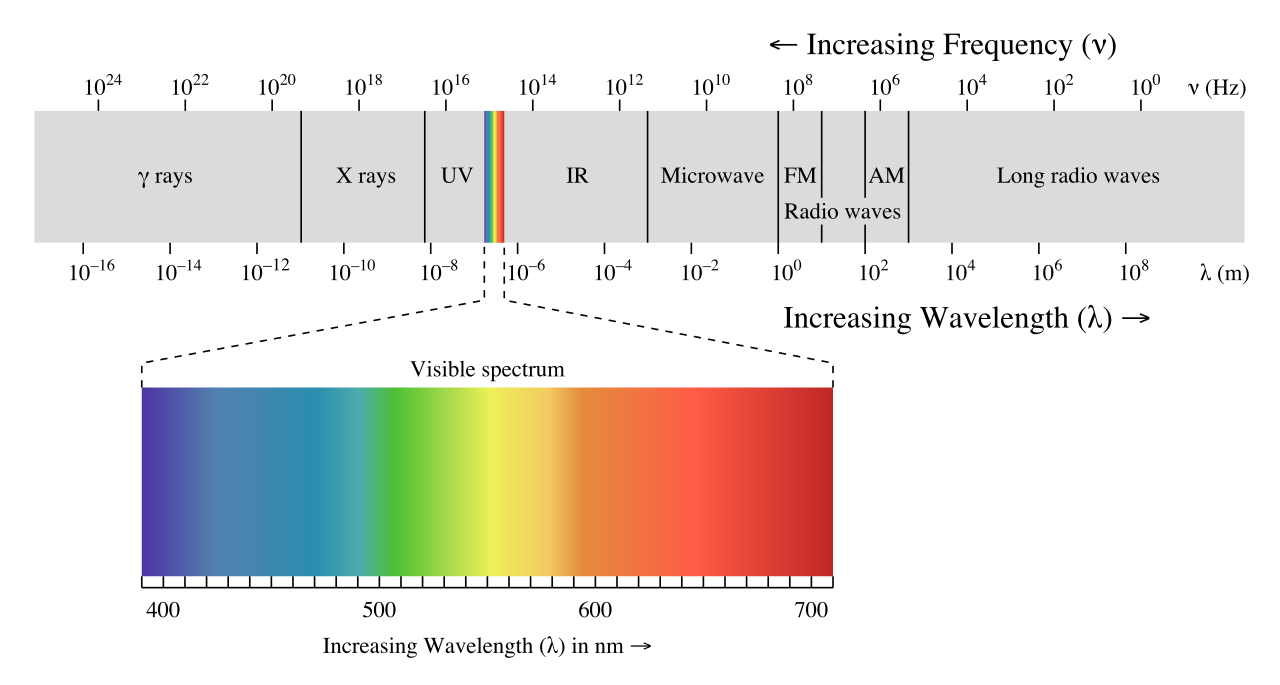
\includegraphics[height=2.25in]{images/em_spectrum.png}}
%    \put(120, 240){\begin{minipage}[t]{0.7 \linewidth}
%    \begin{itemize}
%    \end{itemize}
%    \end{minipage}}
\end{picture}
\end{frame}




\section{What is a Star?}

\begin{frame}
\frametitle{What is a Star?}
\begin{picture}(320,250) 
    % http://large.stanford.edu/courses/2011/ph241/olson1/
    \put(-35, 50){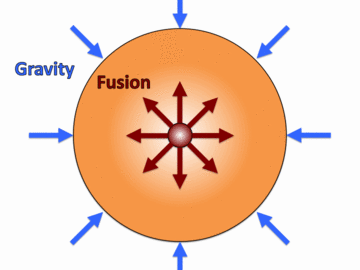
\includegraphics[height=2.15in]{images/force_diagram.eps}}
    \put(130, 220){\begin{minipage}[t]{0.7 \linewidth}
    \begin{itemize}
        \item Gas - primarily hydrogen and helium
        \bigskip
        \pause
        \item Gravitationaly bound 
        \bigskip
        \pause 
        \item Dense and hot enough for nuclear fusion 
    \end{itemize}
    \end{minipage}}
\end{picture}
\end{frame}


\begin{frame}
\frametitle{What is Nuclear Fusion?}
\begin{picture}(320,250) 
    \put(-20, 78){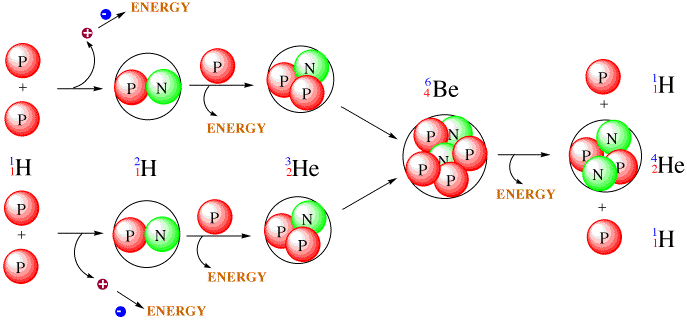
\includegraphics[height=2.25in]{images/Hcycle.eps}}
%    \put(120, 240){\begin{minipage}[t]{0.7 \linewidth}
%    \begin{itemize}
%    \end{itemize}
%    \end{minipage}}
\end{picture}
\end{frame}


\begin{frame}
\frametitle{What is Nuclear Fusion?}
% https://phys.libretexts.org/Bookshelves/University_Physics/Book%3A_University_Physics_(OpenStax)/Map%3A_University_Physics_III_-_Optics_and_Modern_Physics_(OpenStax)/10%3A__Nuclear_Physics/10.2%3A_Nuclear_Binding_Energy
\begin{picture}(320,250) 
    \put(20, 68){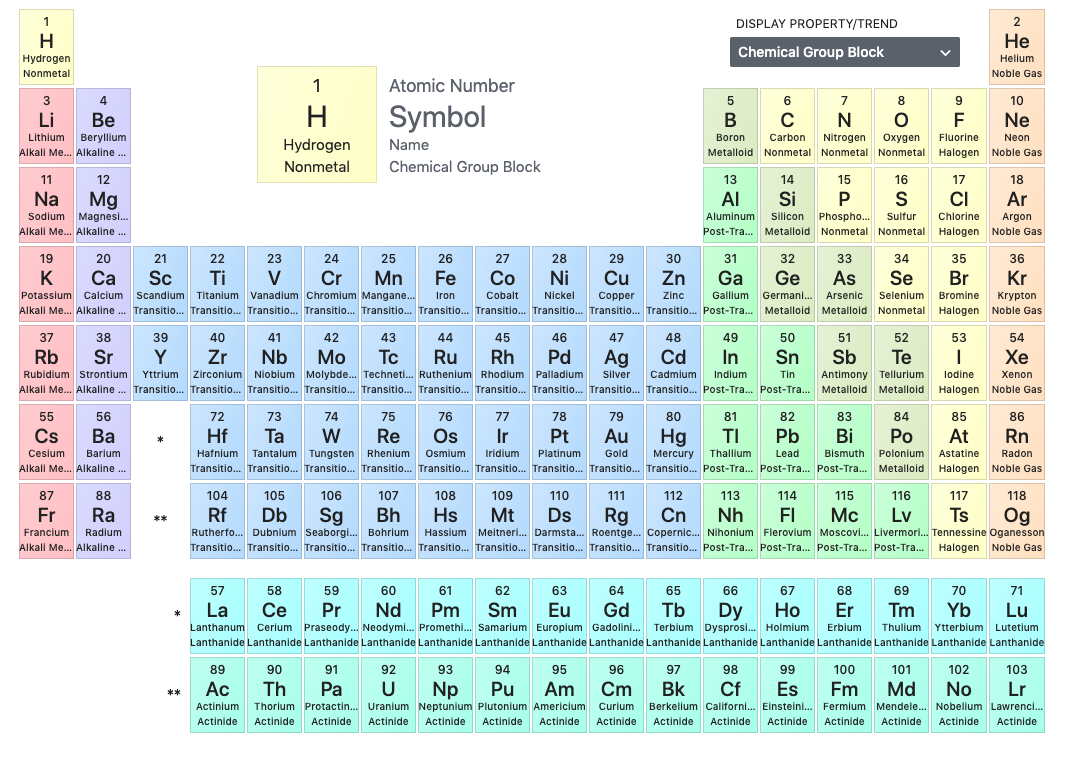
\includegraphics[height=2.5in]{images/periodic_table.png}}
%    \put(120, 240){\begin{minipage}[t]{0.7 \linewidth}
%    \begin{itemize}
%    \end{itemize}
%    \end{minipage}}
\end{picture}
\end{frame}




\begin{frame}
\frametitle{What is Nuclear Fusion?}
% https://phys.libretexts.org/Bookshelves/University_Physics/Book%3A_University_Physics_(OpenStax)/Map%3A_University_Physics_III_-_Optics_and_Modern_Physics_(OpenStax)/10%3A__Nuclear_Physics/10.2%3A_Nuclear_Binding_Energy
\begin{picture}(320,250) 
    \put(20, 68){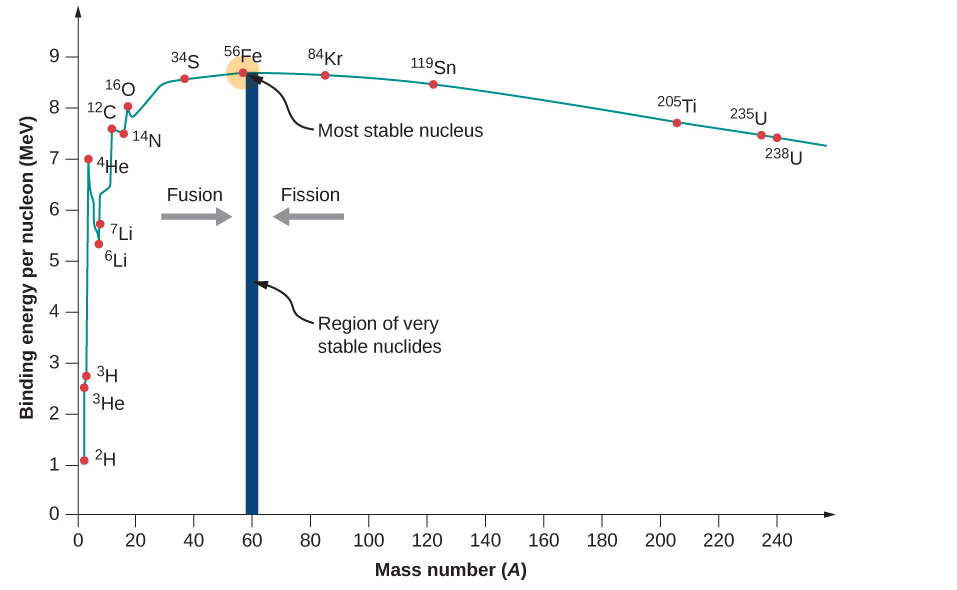
\includegraphics[height=2.5in]{images/nuclear_binding_energy.png}}
%    \put(120, 240){\begin{minipage}[t]{0.7 \linewidth}
%    \begin{itemize}
%    \end{itemize}
%    \end{minipage}}
\end{picture}
\end{frame}



\begin{frame}
\frametitle{Life Cycle of a Star}
Fate determined by :
\bigskip
\begin{itemize}
    \item Mass
    \pause
    \bigskip
    \item Chemical composition
    \pause
    \bigskip
    \item Binary Status
\end{itemize}
\end{frame}

\begin{frame}
\frametitle{Life Cycle of a Star}
\begin{picture}(320,250) 
    %http://astronomy.swin.edu.au/cosmos/H/Hertzsprung-Russell+Diagram
    %By ESO - https://www.eso.org/public/images/eso0728c/, CC BY 4.0, https://commons.wikimedia.org/w/index.php?curid=19915788
    %\put(30, 38){\includegraphics[height=3in]{/Users/asnedden/Projects/NCH/Documents/Talks/Nerd_Hour_09_13_2019/images/hrdiagram1.eps}}
    \put(30, 38){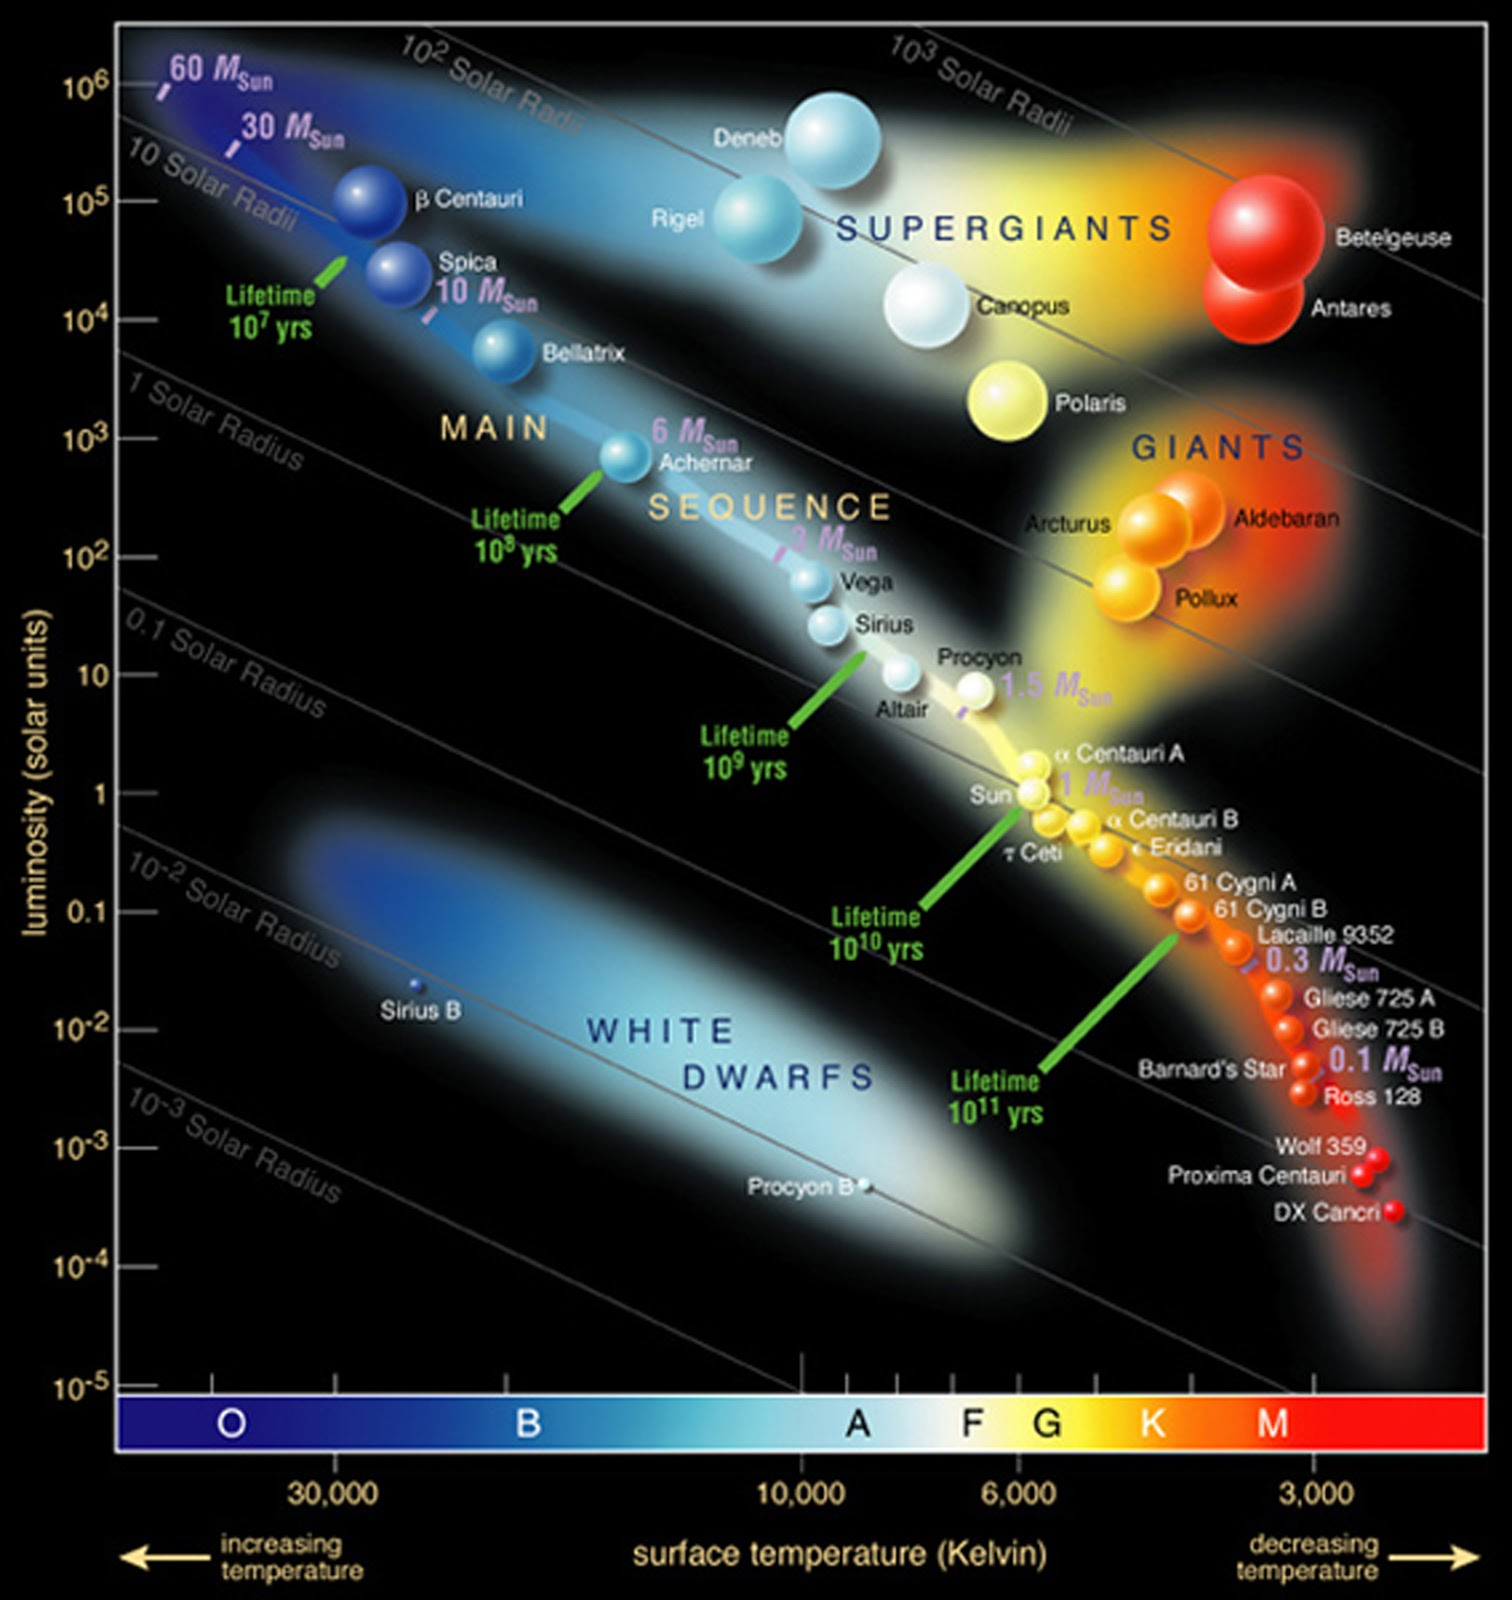
\includegraphics[height=3in]{images/Hertzsprung-Russel_StarData.eps}}
\end{picture}
\end{frame}


\begin{frame}
\frametitle{Life Cycle of a Star}
Life Cycle:
\smallskip
\begin{itemize}
    \item Massive Stars (Mass $> 8 M_{\odot}$ )
    \smallskip
        \pause
        \begin{itemize}
            \item Exist millions of years 
            \pause
            \smallskip
            \item Creates elements up to Iron (during regular burning)
            \pause
            \smallskip
            \item Core-Collapse Supernovae 
            \begin{itemize}
                \pause
                \smallskip
                \item Neutron Star
                \pause
                \smallskip
                \item Black Hole
            \end{itemize}
        \end{itemize}
    \smallskip
    \pause
    \item Regular Stars (Mass $< 8 M_{\odot}$ )
        \pause
        \begin{itemize}
            \item Exist (up to) billions of years before 
            \pause
            \smallskip
            \item Creates lighter elements during regular burning (e.g. Carbon, Oxygen)
            \pause
            \smallskip
            \item Red Giant then planetary nebulae
            \pause
            \smallskip
            \item White Dwarf
            \begin{itemize}
                \pause
                \smallskip
                \item If in binary system - maybe Type Ia supernova
            \end{itemize}
        \end{itemize}
\end{itemize}
\end{frame}


\begin{frame}
\frametitle{Life Cycle of a Star}
\begin{picture}(320,250) 
    % https://www.schoolsobservatory.org/learn/astro/stars/cycle
    \put(0, 78){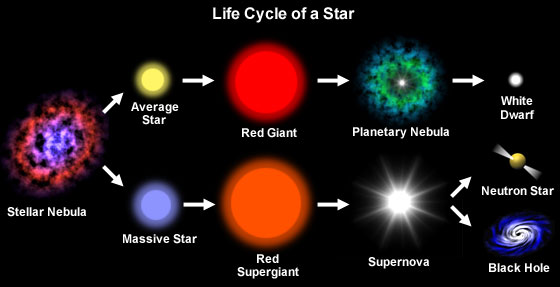
\includegraphics[height=2.25in]{images/starcycle.eps}}
    %\put(-10, 108){\includegraphics[height=1.75in]{/Users/asnedden/Projects/NCH/Documents/Talks/Nerd_Hour_2_11_17/figures/Tycho-supernova-xray.eps}}     % Crab Nebula = 
\end{picture}
\end{frame}


\section{Stellar Remnants}


\begin{frame}
\frametitle{White Dwarf}
\begin{picture}(320,250) 
    %https://imagine.gsfc.nasa.gov/science/objects/dwarfs1.html
    %\put(-35, 70){\includegraphics[height=2.15in]{images/sirius.eps}}
    % By NASA, ESA, H. Bond (STScI), and M. Barstow (University of Leicester) - http://www.spacetelescope.org/images/heic0516a/, CC BY 3.0, https://commons.wikimedia.org/w/index.php?curid=477445
    \put(-35, 70){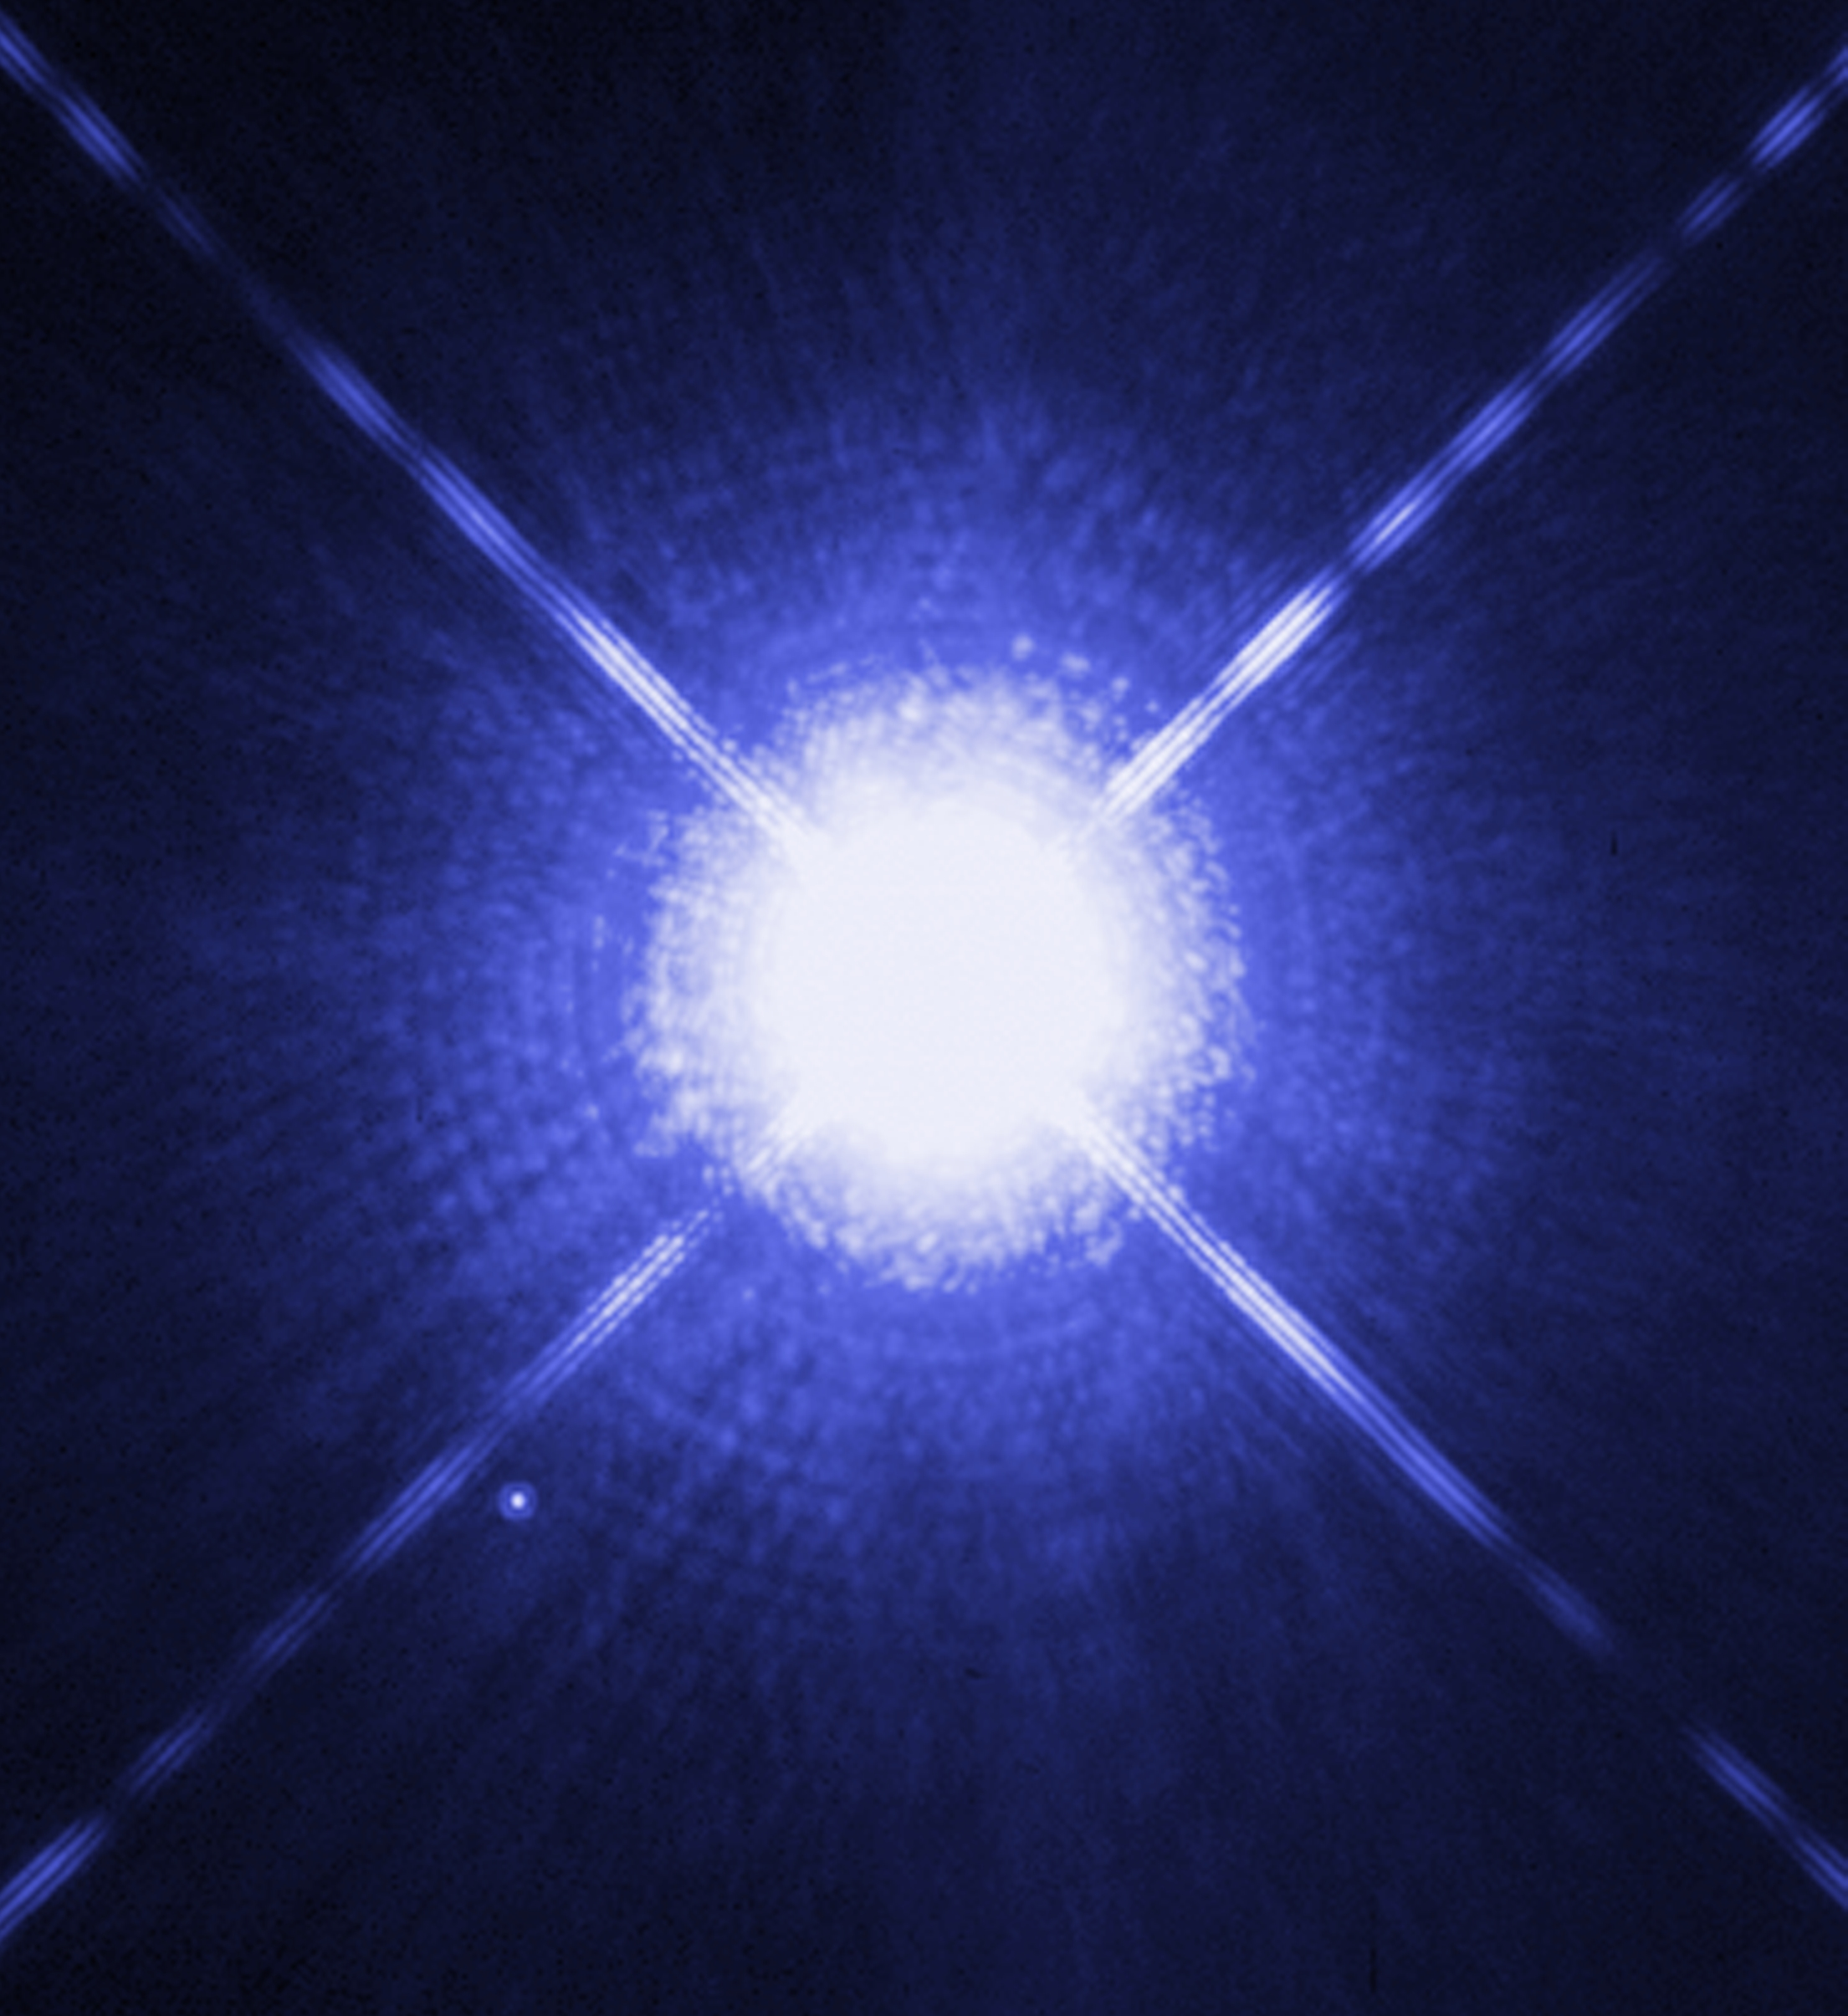
\includegraphics[height=2.15in]{images/Sirius_A_and_B_Hubble_photo.eps}}
    \put(0, 50){\begin{minipage}[t]{0.7 \linewidth}
        Sirius A $\&$ B
    \end{minipage}}
       
    \put(100, 220){\begin{minipage}[t]{0.7 \linewidth}
        \begin{itemize}
            \item No nuclear fusion occuring
            \medskip
            \pause
            \item About size of the earth and mass of the sun.
            \medskip
            \pause
            \begin{itemize}
                \item Density $\sim 10^{6} g/cm^{3}$    % 5.7x10**6
            \end{itemize}
            \medskip
            \pause 
            \item Composed of light elements (e.g. Carbon, Oxygen)
            \medskip
            \pause 
            \item Held up by electron degeneracy pressure
            \begin{itemize}
                \pause
                \item Recall Pauli exclusion principle?
            \end{itemize}
            \medskip
        \end{itemize}
    \end{minipage}}
\end{picture}
\end{frame}


\begin{frame}
\frametitle{White Dwarf}
\begin{picture}(320,250) 
    %https://imagine.gsfc.nasa.gov/science/objects/dwarfs1.html
    \put(10, 60){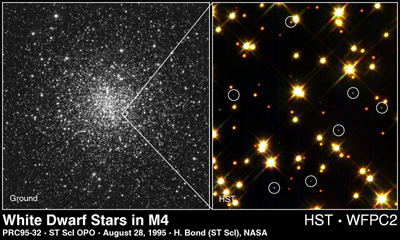
\includegraphics[height=2.4in]{images/m4wd.eps}}
    \put(90, 240){\begin{minipage}[t]{0.7 \linewidth}
       M4 - a globular cluster
    \end{minipage}}
\end{picture}
\smallskip
\end{frame}



\begin{frame}
\frametitle{Neutron Star}
\begin{picture}(320,250) 
%    % By NASA, ESA, H. Bond (STScI), and M. Barstow (University of Leicester) - http://www.spacetelescope.org/images/heic0516a/, CC BY 3.0, https://commons.wikimedia.org/w/index.php?curid=477445
%    %\put(-35, 70){\includegraphics[height=2.15in]{images/sirius.eps}}
    \put(-75, 40){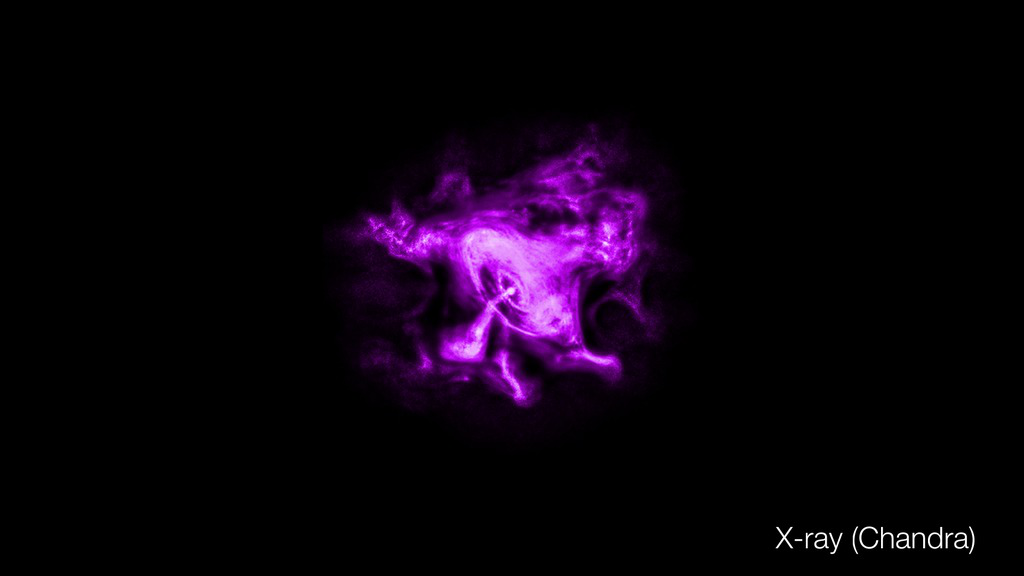
\includegraphics[height=1.35in]{images/crab_nebula_xray.eps}}
    \put(-75, 150){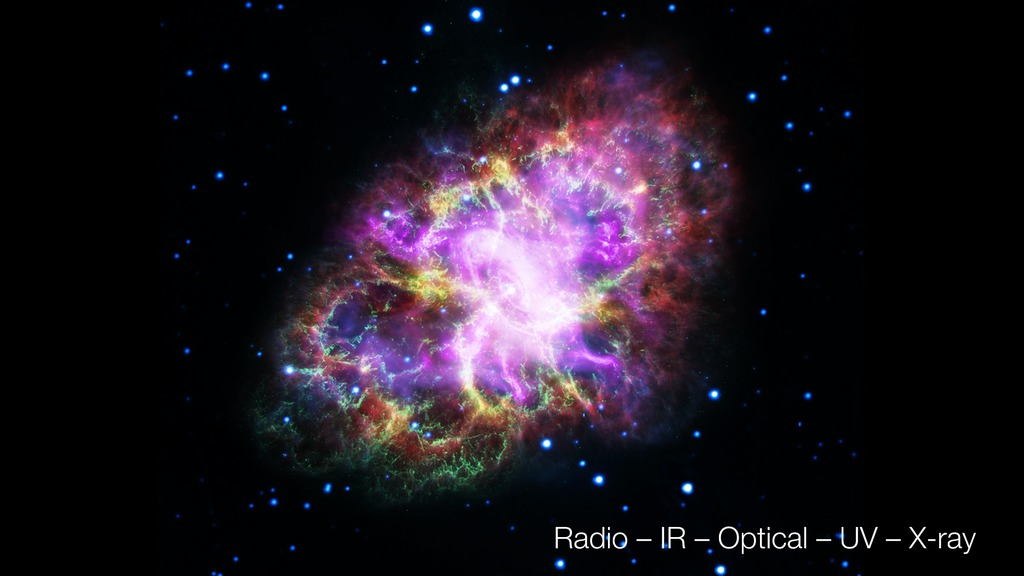
\includegraphics[height=1.35in]{images/crab_nebula_composite.eps}}
    \put(0, 140){\begin{minipage}[t]{0.7 \linewidth}
        {\small Crab Nebula - 1054}
    \end{minipage}}
       
    \put(120, 220){\begin{minipage}[t]{0.7 \linewidth}
        \begin{itemize}
            \item No nuclear fusion occuring
            \medskip
            \pause
            \item Size of Chicago, mass of sun
            \medskip
            \pause
            \begin{itemize}
                \item Density $\sim 10^{14} g/cm^{3}$  % compute 1.5x10**15
            \end{itemize}
            \medskip
            \pause 
            \item Largest nuclei in the universe
            \medskip
            \pause 
            % Cite : http://www.if.ufrgs.br/hadrons/reisenegger1.pdf
            %      : http://adsabs.harvard.edu/full/2001ASPC..248..469R
            \item Magnetic fields of $10^{4}-10^{11} Tesla$
            \begin{itemize}
                \pause
                \item Compare with MRI at 3 Tesla
            \end{itemize}
            \medskip
            \pause 
            \item Held up by neutron degeneracy pressure
            \medskip
            \begin{itemize}
                \pause
                \item Recall Pauli exclusion principle?
            \end{itemize}
            \medskip
        \end{itemize}
    \end{minipage}}
\end{picture}
\end{frame}


\begin{frame}
\frametitle{Neutron Star}
Crab Nebula
\bigskip
\begin{itemize}
    \item Rotates 'slowly' at 30Hz
    \bigskip
    \pause
%https://www.mmto.org/node/675
    \item \href{https://www.dropbox.com/s/njw160luy9eb0kv/CrabPulsarResampled.mp4?dl=0}{\beamergotobutton{Crab Nebula Pulsar - MMT Observatory}}
\end{itemize}
\end{frame}


\begin{frame}
\frametitle{Black Hole}  
% Show video of MW central black hole. M87
\begin{picture}(320,250) 
    %https://www.nasa.gov/feature/goddard/2017/messier-87
    \put(-30, 40){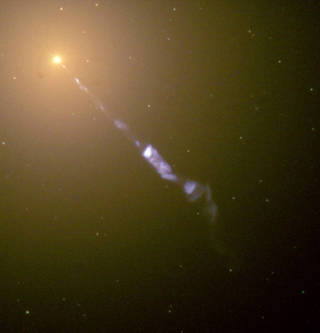
\includegraphics[height=1.35in]{images/m87.eps}}
    \put(-75, 150){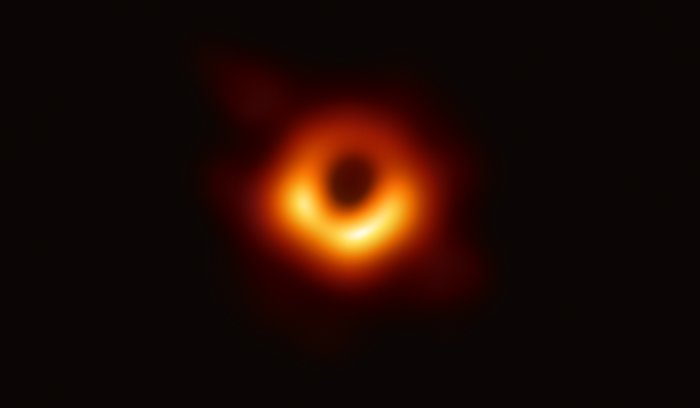
\includegraphics[height=1.35in]{images/m87_event_horizon.eps}}
    \put(0, 140){\begin{minipage}[t]{0.7 \linewidth}
        {\small M87}
    \end{minipage}}
    \put(120, 220){\begin{minipage}[t]{0.7 \linewidth}
    \begin{itemize}
        \item Super-massive blackholes
        \begin{itemize}
            \pause
            \item Probably NOT a stellar remnant
            \pause 
            \item Mass $\sim 10^{6}-10^{9} M_{\odot}$ 
            \pause 
            \item Accrete material. Some of the brightest objects in universe
            \pause 
            \item Has an `observable' event horizon. Not even light can escape
            \pause 
            \item \href{https://www.youtube.com/watch?v=TF8THY5spmo}{\beamergotobutton{Milky Way Supermassive Black Hole - ESO}}
        \end{itemize}
    \end{itemize}
    \end{minipage}}
\end{picture}
\smallskip
\end{frame}


\begin{frame}
\frametitle{Black Hole}  
% Show video of MW central black hole. M87
\begin{picture}(320,250) 
    % By ESA - European Homepage for the NASA/ESA Hubble Space Telescope: [1], Copyrighted free use, https://commons.wikimedia.org/w/index.php?curid=6707568
    \put(-25, 150){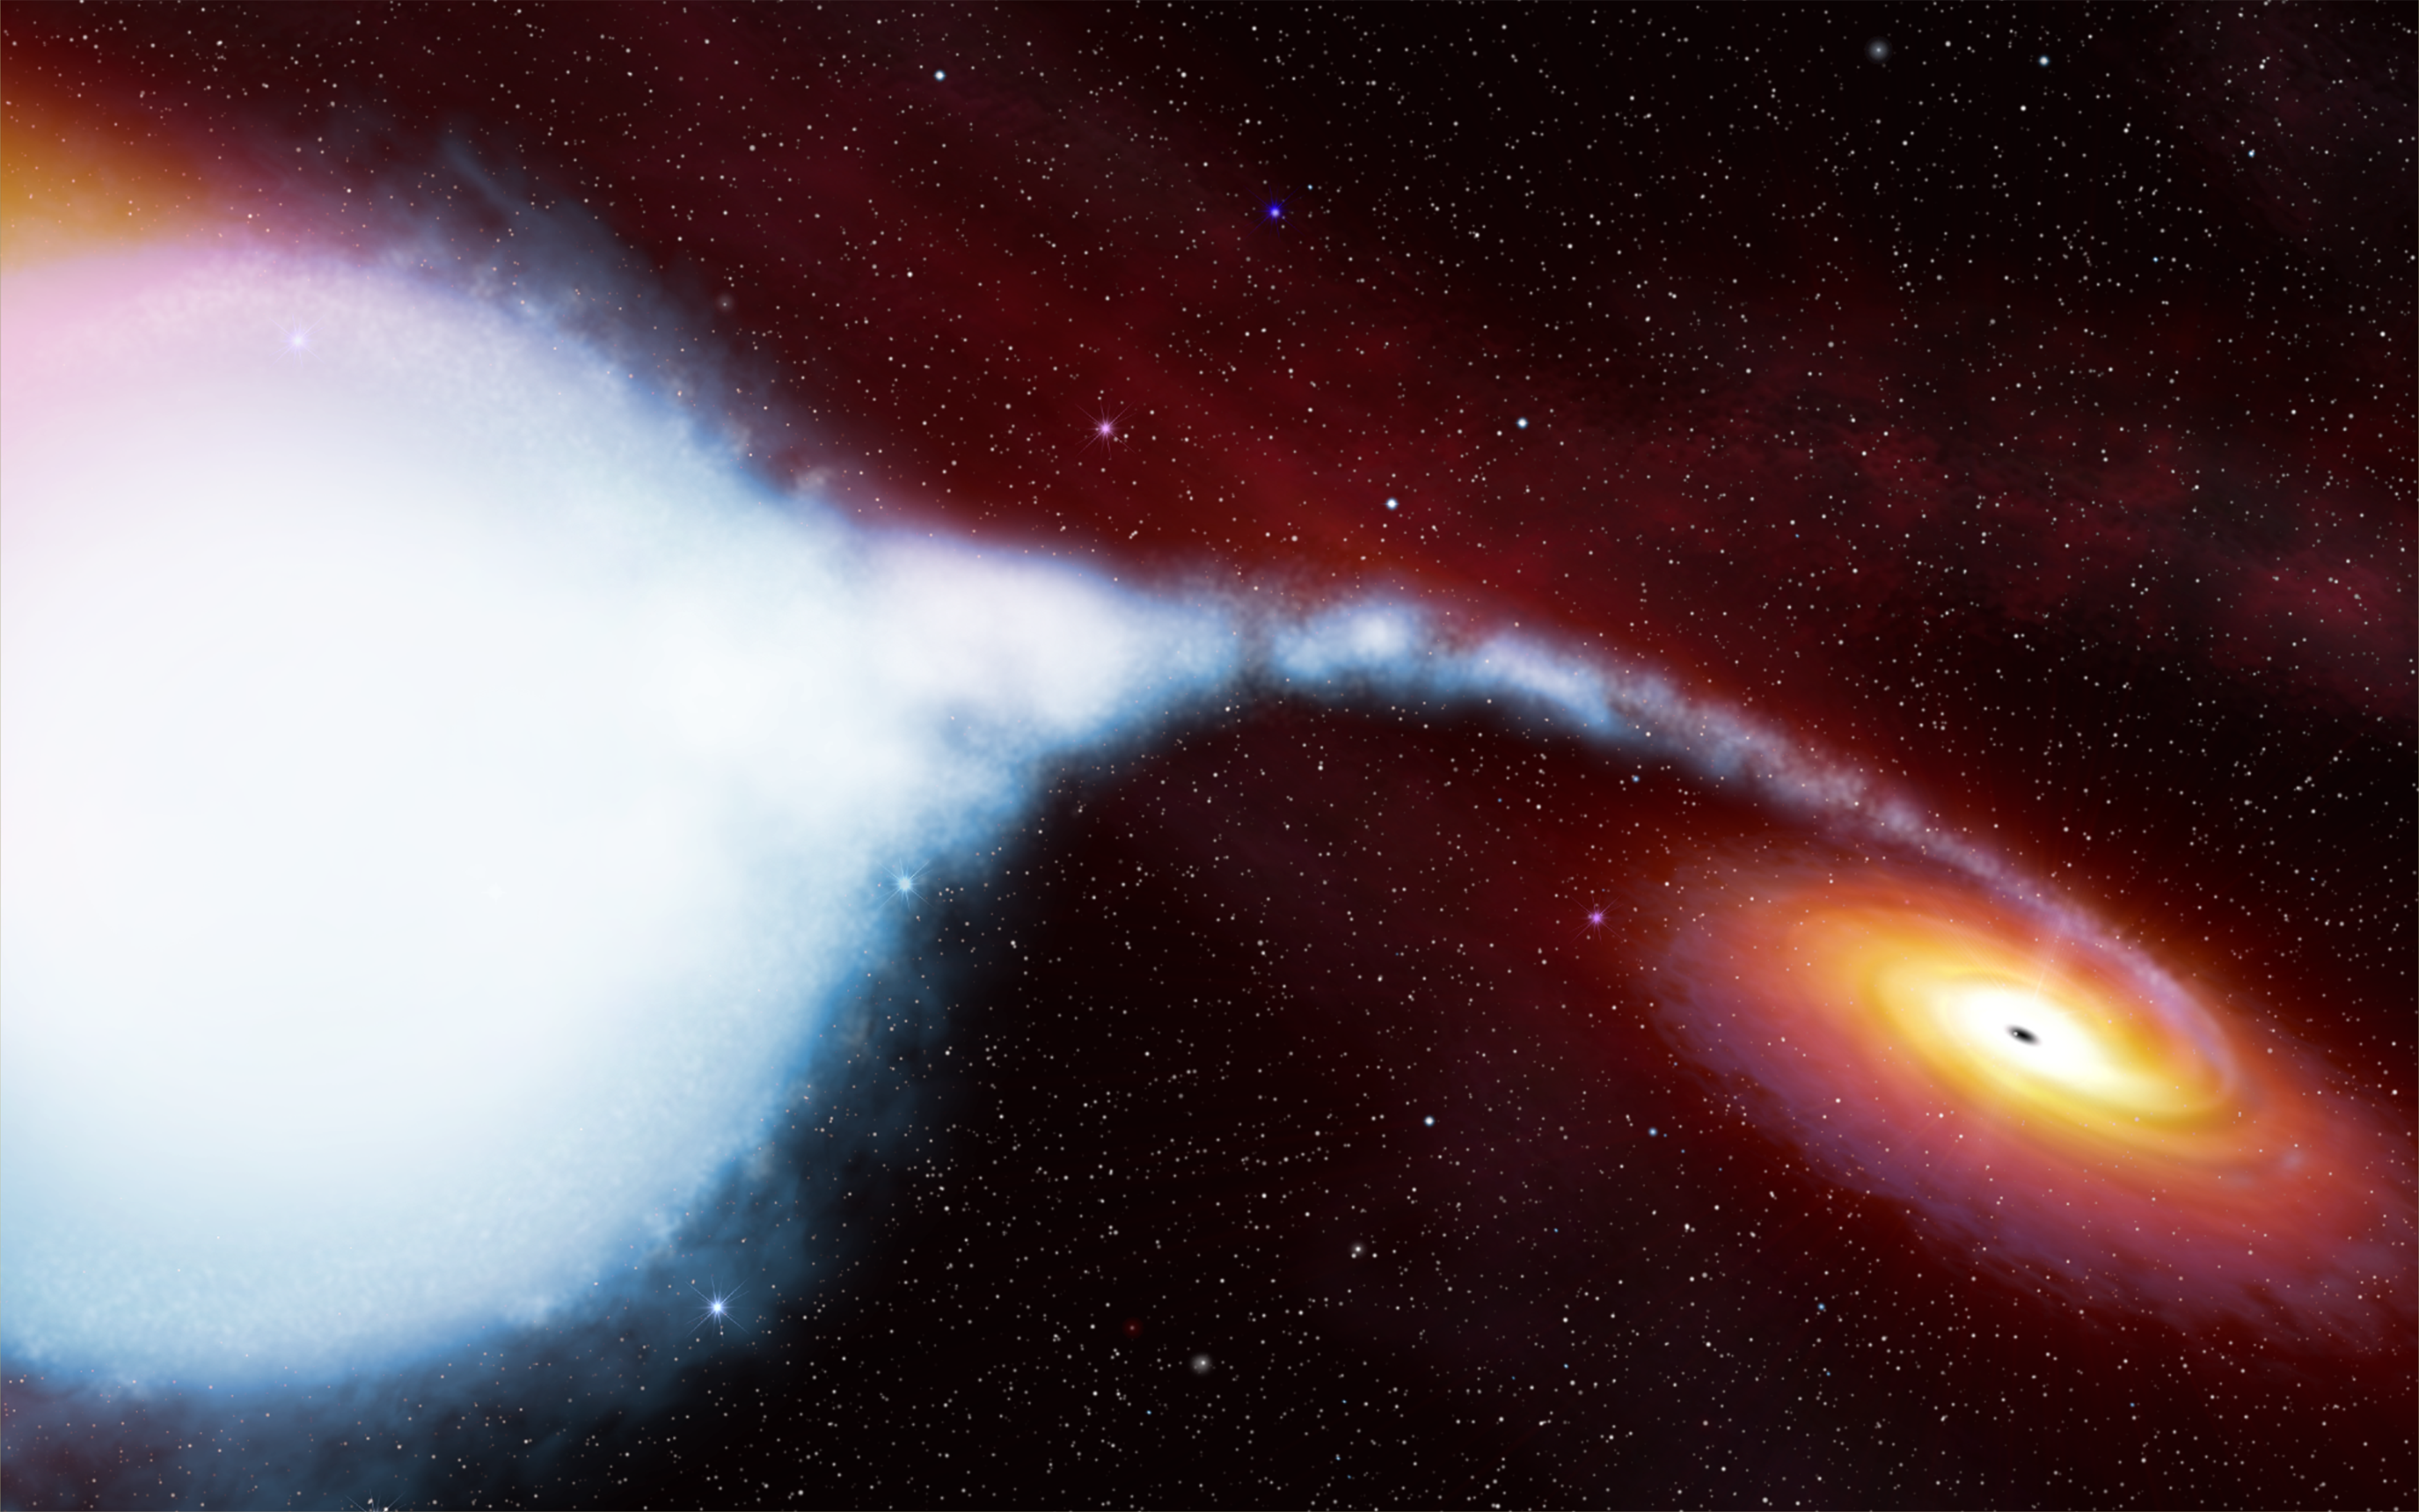
\includegraphics[height=1.25in]{images/cygx1_synth.png}}
    % https://chandra.harvard.edu/photo/2011/cygx1/cygx1_xray.jpg
    \put(-30, 40){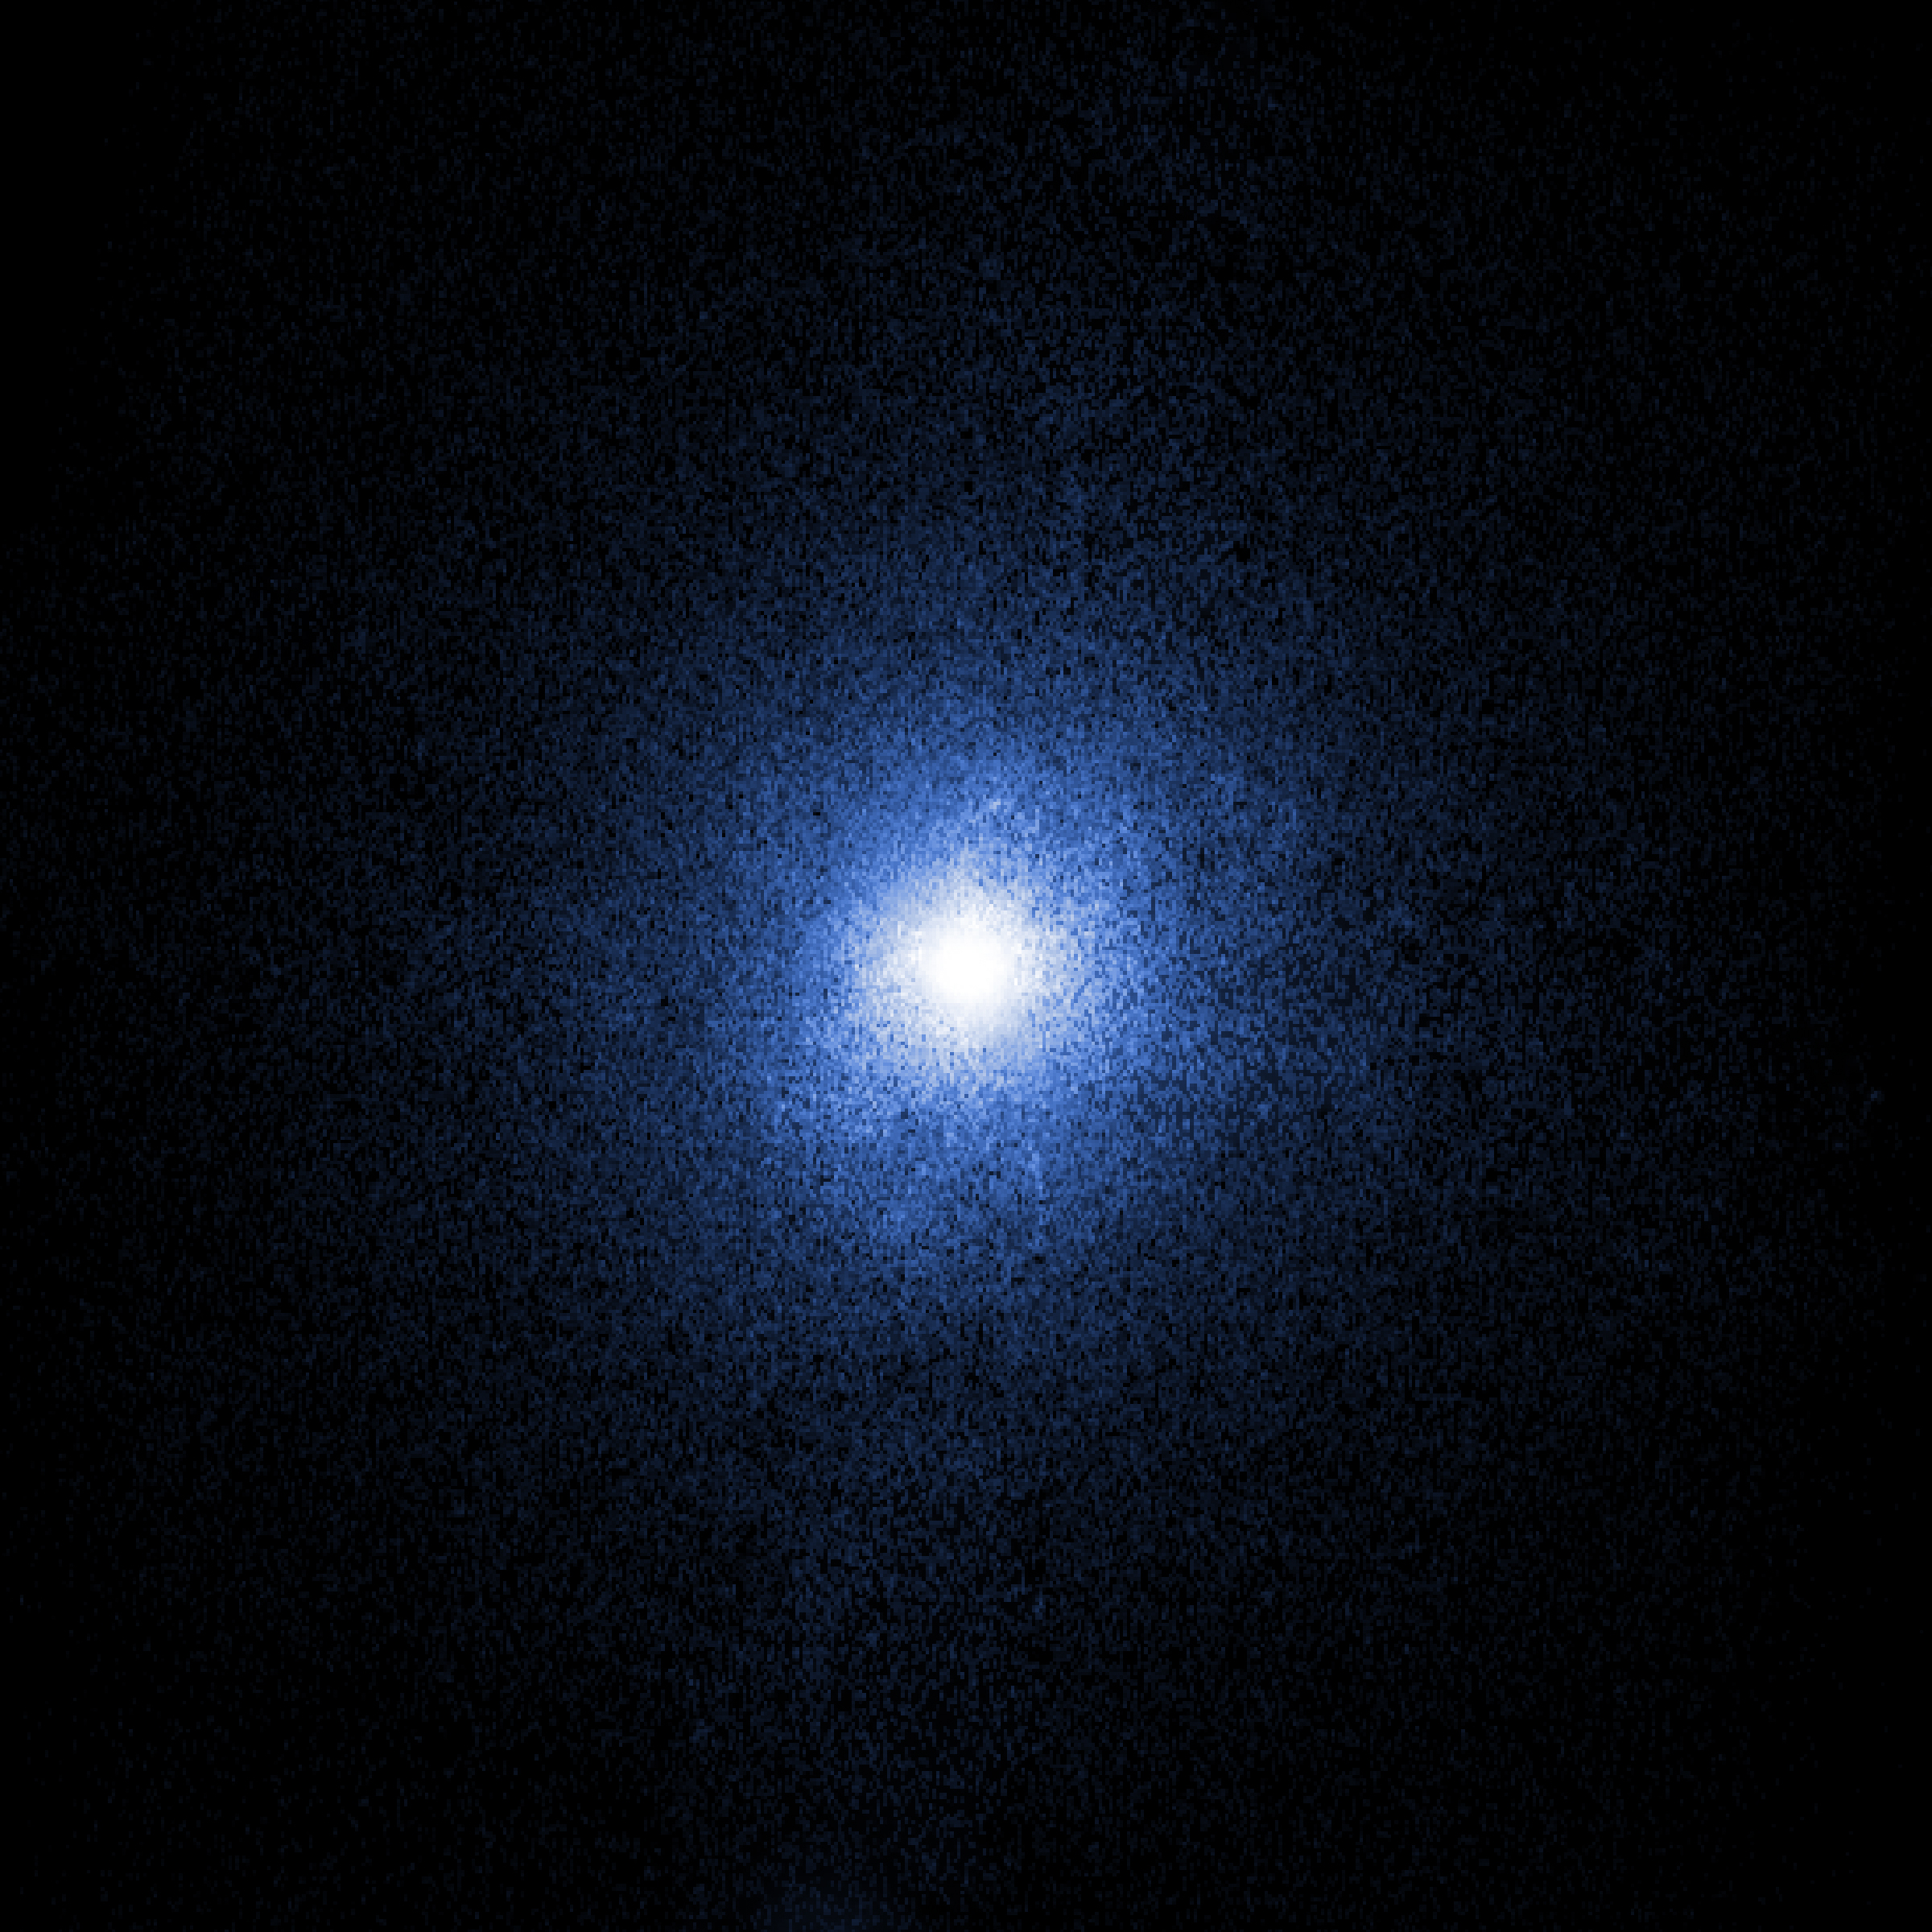
\includegraphics[height=1.35in]{images/cygx1_xray.jpg}}
    % https://www.eso.org/public/images/eso1907a/
    \put(0, 140){\begin{minipage}[t]{0.7 \linewidth}
        {\small Cygnus X-1}
    \end{minipage}}
    \put(120, 220){\begin{minipage}[t]{0.7 \linewidth}
    \begin{itemize}
        \item Super-massive blackholes
        \begin{itemize}
            \item Probably NOT a stellar remnant
            \item Mass $\sim 10^{6}-10^{9} M_{\odot}$ 
            \item Accrete material. Some of the brightest objects in universe
            \item Has an 'observable' event horizon. Not even light can escape
            \item \href{https://www.youtube.com/watch?v=TF8THY5spmo}{\beamergotobutton{Milky Way Supermassive Black Hole - ESO}}
        \end{itemize}
        \item Stellar mass blackholes 
        \pause
        \begin{itemize}
            \item Likely stellar remnants
            \pause 
            \item Mass $\sim 4-20 M_{\odot}$ 
            \pause 
            \item Often observed as a `dark' companion in a binary system
            \pause 
            \item Can also acrete material
        \end{itemize}
    \end{itemize}
    \end{minipage}}
\end{picture}
\smallskip
\end{frame}


\section{Multi-Messenger Astronomy}
\begin{frame}
\frametitle{The Detector}
% Show video of MW central black hole. M87
\begin{picture}(320,250) 
    \put(-30, 40){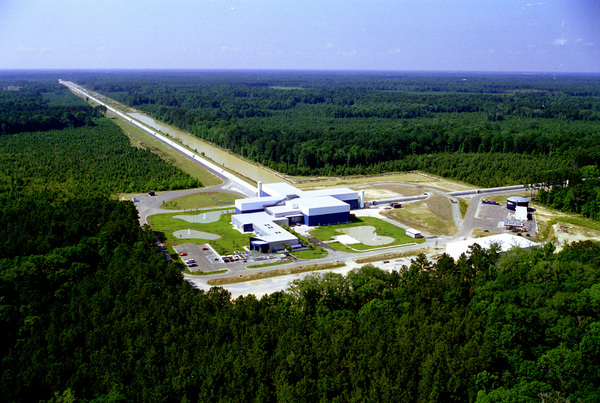
\includegraphics[height=1.10in]{images/ligo_livingston.jpg}}
    %https://journals.aps.org/prl/abstract/10.1103/PhysRevLett.116.061102
    \put(-25, 150){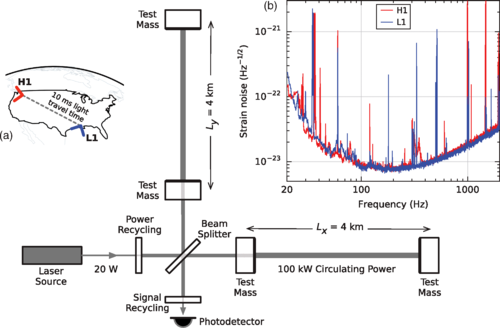
\includegraphics[height=1.10in]{images/ligo_setup.eps}}
    \put(120, 220){\begin{minipage}[t]{0.7 \linewidth}
    LIGO : Laser Interferometer Gravitational-Wave Observatory 
    \pause
    \begin{itemize}
        \item 2 locations
        \pause
        \begin{itemize}
            \item Hanford, Washington
            \pause
            \item Livingston, Louisiana
        \end{itemize}
        \pause
        \item L - shaped
        \pause
        \begin{itemize}
            \item 4km per leg.
        \end{itemize}
        \pause
        \item Sensitive
        \pause
        \begin{itemize}
            \item Can measure distortions in space-time at $10^{-18}m$
        \end{itemize}
    \end{itemize}
    \end{minipage}}
\end{picture}
\smallskip

\end{frame}




\begin{frame}
\frametitle{First Detection - 2015}
% Show video of MW central black hole. M87
\begin{picture}(320,250) 
    \put(50, 50){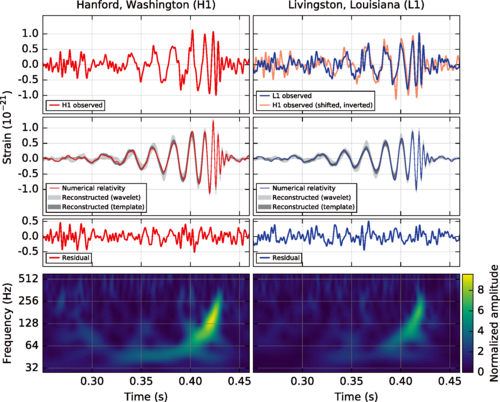
\includegraphics[height=2.40in]{images/ligo_first_detection.png}}
    %https://journals.aps.org/prl/abstract/10.1103/PhysRevLett.116.061102
    \put(70, 240){\begin{minipage}[t]{0.7 \linewidth}
    A black hole merger - $36M_{\odot} + 29M_{\odot}$  
    \end{minipage}}
\end{picture}
\end{frame}


\begin{frame}
\frametitle{First Detection - 2015}
% Show video of MW central black hole. M87
\begin{picture}(320,250) 
    \put(50, 50){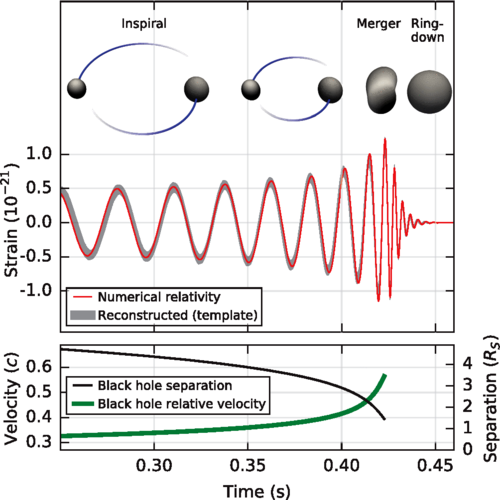
\includegraphics[height=2.40in]{images/ligo_first_detection_2.png}}
    %https://journals.aps.org/prl/abstract/10.1103/PhysRevLett.116.061102
    \put(70, 240){\begin{minipage}[t]{0.7 \linewidth}
    A black hole merger - $36M_{\odot} + 29M_{\odot}$  
    \end{minipage}}
\end{picture}
\end{frame}



\begin{frame}
\frametitle{First Detection - 2015}
% Show video of MW central black hole. M87
\begin{picture}(320,250) 
    \put(70, 240){\begin{minipage}[t]{0.7 \linewidth}
    A black hole merger - $36M_{\odot} + 29M_{\odot}$  
    \end{minipage}}
    \put(120, 150){\begin{minipage}[t]{0.7 \linewidth}
    \href{https://www.youtube.com/watch?v=QyDcTbR-kEA}{\beamergotobutton{The Chirp}}
    \end{minipage}}
\end{picture}
\end{frame}

% Neutron Star merger Notes
% http://adsabs.harvard.edu/abs/2017PhRvL.119p1101A
% http://adsabs.harvard.edu/abs/2017ApJ...848L..13A
% http://adsabs.harvard.edu/abs/2017ApJ...848L..12A
%
\begin{frame}
\frametitle{Neutron Star Merger (GW170817) - 2017}
% Show video of MW central black hole. M87
    %\put(70, 240){\begin{minipage}[t]{0.7 \linewidth}
    %A black hole merger - $36M_{\odot} + 29M_{\odot}$  
    %\end{minipage}}
    Measured :
    \begin{itemize}
        \item 100s long gravitational wave signal (Livingston, Hanford, Virgo), followed by
        \pause
        \item Short gamma ray burst - measured by Fermi space telescope
        \pause
        \item Kilonova powered by radioactive decay of r-process nuclei
        \pause
        \item 3 gravitational wave detectors (2 LIGO, 1 VIRGO) located it on sky
        \pause
        \item Confirmed by xray, ultra-violet, optical, infrared and radio  measurements
        \pause
        \item Estimated distance of $120 \times 10^{6}$ light years.
        \pause
        \begin{itemize}
            \item Independently confirmed by both optical and gravitational wave observations.
        \end{itemize}
    \end{itemize}
\end{frame}


\begin{frame}
\frametitle{Neutron Star Merger (GW170817) - 2017}
% Show video of MW central black hole. M87
\begin{picture}(320,250) 
    %\put(70, 240){\begin{minipage}[t]{0.7 \linewidth}
    \put(20, 50){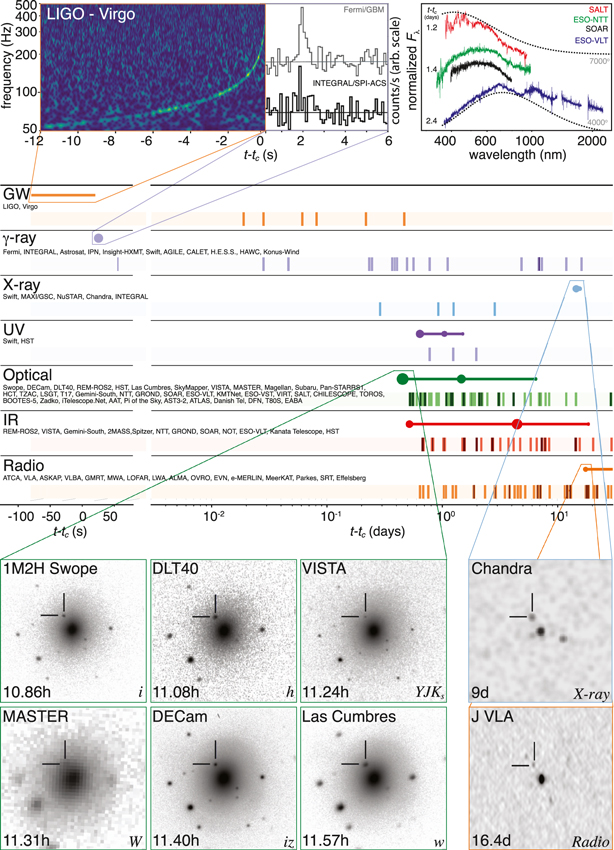
\includegraphics[height=2.750in,width=3.25in]{images/neutron_star_merger_timeline.jpg}}
    %A black hole merger - $36M_{\odot} + 29M_{\odot}$  
    %\end{minipage}}
    %\put(120, 150){\begin{minipage}[t]{0.7 \linewidth}
    %Timeline
    %\end{minipage}}
\end{picture}
\end{frame}


\begin{frame}
\frametitle{Neutron Star Merger (GW170817) - 2017}
% Show video of MW central black hole. M87
\begin{picture}(320,250) 
    %\put(70, 240){\begin{minipage}[t]{0.7 \linewidth}
    % By Hubble Space Telescope, NASA and ESA - https://www.nasa.gov/press-release/nasa-missions-catch-first-light-from-a-gravitational-wave-event, Public Domain, https://commons.wikimedia.org/w/index.php?curid=63409545
    \put(60, 50){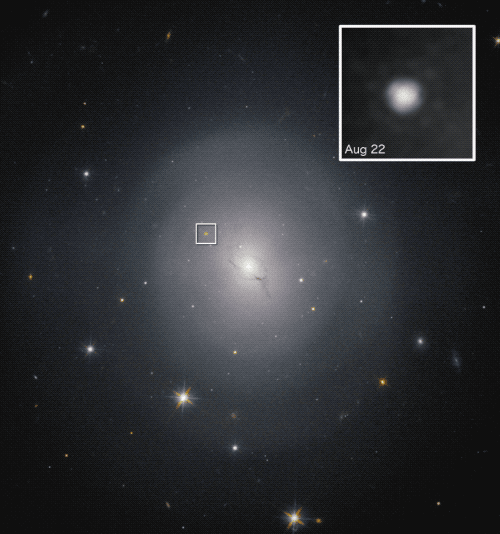
\includegraphics[height=2.750in]{images/NGC_4993-0.png}}
    %A black hole merger - $36M_{\odot} + 29M_{\odot}$  
    %\end{minipage}}
    %\put(120, 150){\begin{minipage}[t]{0.7 \linewidth}
    %Timeline
    %\end{minipage}}
\end{picture}
\end{frame}

\begin{frame}
\frametitle{Neutron Star Merger (GW170817) - 2017}
% Show video of MW central black hole. M87
\begin{picture}(320,250) 
    %\put(70, 240){\begin{minipage}[t]{0.7 \linewidth}
    % By Hubble Space Telescope, NASA and ESA - https://www.nasa.gov/press-release/nasa-missions-catch-first-light-from-a-gravitational-wave-event, Public Domain, https://commons.wikimedia.org/w/index.php?curid=63409545
    \put(60, 50){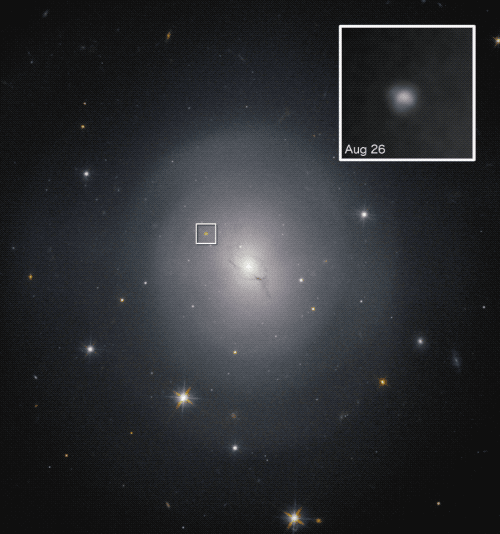
\includegraphics[height=2.750in]{images/NGC_4993-1.png}}
    %A black hole merger - $36M_{\odot} + 29M_{\odot}$  
    %\end{minipage}}
    %\put(120, 150){\begin{minipage}[t]{0.7 \linewidth}
    %Timeline
    %\end{minipage}}
\end{picture}
\end{frame}


\begin{frame}
\frametitle{Neutron Star Merger (GW170817) - 2017}
% Show video of MW central black hole. M87
\begin{picture}(320,250) 
    %\put(70, 240){\begin{minipage}[t]{0.7 \linewidth}
    % By Hubble Space Telescope, NASA and ESA - https://www.nasa.gov/press-release/nasa-missions-catch-first-light-from-a-gravitational-wave-event, Public Domain, https://commons.wikimedia.org/w/index.php?curid=63409545
    \put(60, 50){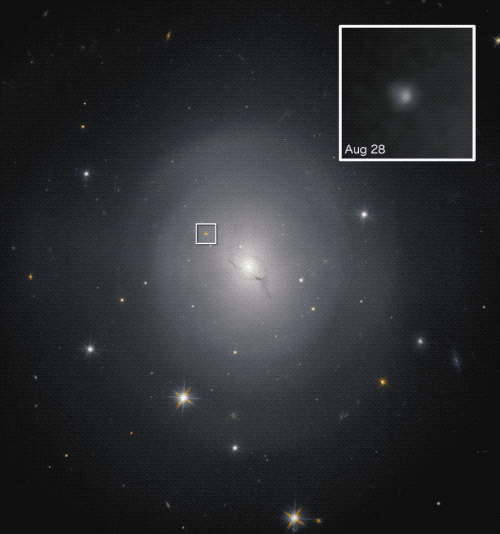
\includegraphics[height=2.750in]{images/NGC_4993-2.png}}
    %A black hole merger - $36M_{\odot} + 29M_{\odot}$  
    %\end{minipage}}
    %\put(120, 150){\begin{minipage}[t]{0.7 \linewidth}
    %Timeline
    %\end{minipage}}
\end{picture}
\end{frame}


\begin{frame}
\frametitle{Neutron Star Merger (GW170817) - 2017}
% Show video of MW central black hole. M87
    %\put(70, 240){\begin{minipage}[t]{0.7 \linewidth}
    %A black hole merger - $36M_{\odot} + 29M_{\odot}$  
    %\end{minipage}}
    Consequences:
    \pause
    \begin{itemize}
        \item Correlation between gravitational and light waves puts limits on the speed of light and gravity waves. 
        \begin{itemize}
            \pause
            \item Fractional difference $= 10^{-15}$
        \end{itemize}
        \pause
        \item Constrains nuclear equation of state.
        \pause
        \item Provided the progenitors for short gamma ray bursts
        \pause
        \item Explains the origins of some heavy elements (e.g. gold, platinum)
    \end{itemize}
\end{frame}



%\end{itemize}
%\end{frame}
%\begin{frame}
%\printbibliography
%% cite B2FH paper
%% cite neutron star merger paper and bh merger paper
%\end{frame}

% Backup slides

%\begin{frame}
%\frametitle{Spare slide : Momentum Conservation}
%\end{frame}

% 1987a : https://chandra.harvard.edu/photo/2017/sn1987a/more.html
% Crab Nebula : Neutron star https://chandra.harvard.edu/photo/1999/0052/, https://svs.gsfc.nasa.gov/30944
% Vela Pulsar : https://svs.gsfc.nasa.gov/cgi-bin/details.cgi?aid=10426
% Elements https://courses.lumenlearning.com/astronomy/chapter/evolution-of-massive-stars-an-explosive-finish/


% To Do:
% 1. Read astronut about stars to enusre I got the physics right.
% 2. Read about nuclear fusion
% 3. Jargon alert? 
% 4. First slide should motivate talk. Why do we care about stars?
% 5. Plot of lifetime vs. mass
% 6. Look up why planetary nebula forms
% 7. Periodic Table
% 8. Bring the Bible and Astronut
% 9. Explain why neutron stars spin




\end{document}
